\documentclass[12pt,a4paper]{article}
\usepackage[utf8]{inputenc}
\usepackage{amsmath}
\usepackage{amsfonts}
\usepackage{amssymb}
\usepackage{graphicx}
\usepackage[left=3cm,right=3cm,top=2.5cm,bottom=2.5cm]{geometry}

% headers / footers
\usepackage{fancyhdr}
	\pagestyle{fancy}
	\fancyhf{}
	\lhead{ENS1161: Computer Fundamentals}
	\rhead{Assignment 1}
	\lfoot{Martin Ponce, ID: 10371381}
	\rfoot{\thepage\ of \pageref*{LastPage}}
	\renewcommand{\footrulewidth}{0.5pt}

% defining landscape headers / footers
\fancypagestyle{fancylscape}{
	\fancyhf{}
	\renewcommand{\footrulewidth}{0pt}
	\renewcommand{\headrulewidth}{0pt}
	% header
	\begin{textblock}{0.05}[-0.5,-2](0,0)
		{\rotatebox{90}{CSG1132: Communicating in an IT Environment}}
	\end{textblock}
		\begin{textblock}{0.05}[-0.5,-1](0,0)
		{\rotatebox{90}{Assignment 1a}}
	\end{textblock}
	\begin{textblock}{0.05}[-1,-0.109](0,0)
		{\rotatebox{90}{\rule{24.2cm}{0.5pt}}}
	\end{textblock}
	% footer
	\begin{textblock}{0.05}[-19,-4.28](0,0)
		{\rotatebox{90}{Martin Ponce, ID: 10371381}}
	\end{textblock}
		\begin{textblock}{0.05}[-19,-12.8](0,0)
		{\rotatebox{90}{\thepage\ of \pageref*{LastPage}}}
	\end{textblock}
		\begin{textblock}{0.05}[-18.7,-0.109](0,0)
		{\rotatebox{90}{\rule{24.2cm}{0.5pt}}}
	\end{textblock}
}

% defining settings for textpos
\usepackage[absolute]{textpos}
\setlength{\TPHorizModule}{\paperwidth}
\setlength{\TPVertModule}{\paperheight}

% creates landscape pages
\usepackage{pdflscape}

% add pages from pdfs
\usepackage{pdfpages}

% adds links to references and colors them blue
\usepackage{hyperref}
\hypersetup{colorlinks=true,
			linkcolor=blue,
			citecolor=blue,
			urlcolor=blue}

% adjusts padding between caption and figure
\setlength{\belowcaptionskip}{10pt}

% last page
\usepackage{lastpage}

% front matter
\title{Edith Cowan University\\ENS1161\\Assignment 1}
\author{Martin Ponce\\ID: 10371381}
\date{August 28, 2014}

\begin{document}

% assignment coversheet
\includepdf{./../img/assignment_coversheet_Ponce_10371381.pdf}

% title page
\newpage
\null  % Empty line
\nointerlineskip  % No skip for prev line
\vfill
\let\snewpage \newpage
\let\newpage \relax
\maketitle
\thispagestyle{empty}
\let \newpage \snewpage
\vfill

% toc
\newpage
\tableofcontents

% page 1
\newpage
\section{Question 1}

\subsection{A) Consider the following argument}
\begin{quote}
If bears are brown then giraffes are not green. If bears are not brown then rabbits are red. Rabbits are red. Therefore giraffes are not green.
\end{quote}

\begin{itemize}
\item $b$ = bears are brown
\item $g$ = giraffes are green
\item $r$ = rabbits are red
\end{itemize}

\subsubsection{State the argument in symbols}
$$b \rightarrow \sim{g}, \sim{b} \rightarrow r, r \mid \sim{g}$$

\subsubsection{Rewrite the symbolic argument as a proposition}
$$(\sim{b} \wedge r) \rightarrow \sim{g}$$

\subsubsection{Construct a truth table for the proposition}
\begin{table}[h]
\centering
\caption{Question 1A Truth Table}
\begin{tabular}{c|c|c|c|c|c}
$b$ & $r$ & $g$ & $\sim{b} \wedge r$ & $\sim{g}$ & $(\sim{b} \wedge r) \rightarrow \sim{g}$ \\
\hline
0 & 0 & 0 & 0 & 1 & 1 \\
\hline
0 & 0 & 1 & 0 & 0 & 1 \\
\hline
0 & 1 & 0 & 1 & 1 & 1 \\
\hline
0 & 1 & 1 & 1 & 0 & 0 \\
\hline
1 & 0 & 0 & 0 & 1 & 1 \\
\hline
1 & 0 & 1 & 0 & 0 & 1 \\
\hline
1 & 1 & 0 & 0 & 1 & 1 \\
\hline
1 & 1 & 1 & 0 & 0 & 1 \\
\hline
\end{tabular}
\end{table}

\subsubsection{State whether the argument is valid}

The proposition is logically equivalent to the argument, as shown in the truth table. Therefore the argument is valid.


\newpage
\subsection{B) The propositions below can be arranged in three groups so that each member of a group is logically equivalent to the other two. Find three groups}

\begin{enumerate}
\item Either the light is not on or the system is ready.
	\begin{itemize}
	\item $\sim{l} \vee s$
	\end{itemize}
\item If the system is ready then the light is on.
	\begin{itemize}
	\item $s \rightarrow l$
	\end{itemize}
\item If the light is on then the system is not ready.
	\begin{itemize}
	\item $l \rightarrow \sim{s}$
	\end{itemize}
\item If the light is not on then the system is not ready.
	\begin{itemize}
	\item $\sim{l} \rightarrow \sim{s}$
	\end{itemize}
\item If the system is not ready then the light is not on.
	\begin{itemize}
	\item $\sim{s} \rightarrow \sim{l}$
	\end{itemize}
\item Either the system is not ready or the light is on.
	\begin{itemize}
	\item $\sim{s} \vee l$
	\end{itemize}
\item If the light is on then the system is ready.
	\begin{itemize}
	\item $l \rightarrow s$
	\end{itemize}
\item If the system is ready then the light is not on.
	\begin{itemize}
	\item $s \rightarrow \sim{l}$
	\end{itemize}
\item Either the system is not ready or the light is not on.
	\begin{itemize}
	\item $\sim{s} \vee \sim{l}$
	\end{itemize}
\end{enumerate}

\newpage
\begin{landscape}
\thispagestyle{fancylscape}
\begin{table}[h]
\centering
\caption{Question 1B Truth Table}
\begin{tabular}{c|c|c|c|c|c|c|c|c|c|c|c|c}
$s$ & $l$ & $\sim{s}$ & $\sim{l}$ & $\sim{l} \vee s$ & $s \rightarrow l$ & $l \rightarrow \sim{s}$ & $\sim{l} \rightarrow \sim{s}$ & $\sim{s} \rightarrow \sim{l}$ & $\sim{s} \vee l$ & $ \rightarrow s$ & $s \rightarrow \sim{l}$ & $\sim{s} \vee \sim{l}$ \\
\hline
0 & 0 & 1 & 1 & 1 & 1 & 1 & 1 & 1 & 1 & 1 & 1 & 1 \\
\hline
0 & 1 & 1 & 0 & 0 & 1 & 1 & 1 & 0 & 1 & 0 & 1 & 1 \\
\hline
1 & 0 & 0 & 1 & 1 & 0 & 1 & 0 & 1 & 0 & 1 & 1 & 1 \\
\hline
1 & 1 & 0 & 0 & 1 & 1 & 0 & 1 & 1 & 1 & 1 & 0 & 0 \\
\hline
\end{tabular}
\end{table}
\end{landscape}

\newpage
\subsubsection{Question 1B Answer}

\begin{table}[h]
\centering
\caption{Group 1}
\begin{tabular}{c|l}
Proposition number & Symbolic \\
\hline
1 & $\sim{l} \vee s$\\
\hline
5 & $\sim{s} \rightarrow \sim{l}$\\
\hline
7 & $l \rightarrow s$\\
\hline
\end{tabular}
\end{table}

\begin{table}[h]
\centering
\caption{Group 2}
\begin{tabular}{c|l}
Proposition number & Symbolic \\
\hline
2 & $s \rightarrow l$ \\
\hline
4 & $\sim{l} \rightarrow \sim{s}$ \\
\hline
6 & $\sim{s} \vee l$ \\
\end{tabular}
\end{table}

\begin{table}[h]
\centering
\caption{Group 3}
\begin{tabular}{c|l}
Proposition number & Symbolic \\
\hline
3 & $l \rightarrow \sim{s}$ \\
\hline
8 & $s \rightarrow \sim{l}$ \\
\hline
9 & $\sim{s} \vee \sim{l}$ \\
\hline
\end{tabular}
\end{table}

\newpage
\section{Question 2}
\begin{quote}
A group of 100 students is polled to see how many watched three TV shows, Action, Buzz, and Calypso. The results showed that:
\begin{itemize}
\item 59 watched Action, denoted by $A$
\item 68 watched Buzz, denoted by $B$
\item 52 watched Calypso, denoted by $C$
\item 41 watched Action and Buzz
\item 34 watched Action and Calypso
\item 38 watched Buzz and Calypso
\item 11 did not watch any of the the three shows 
\end{itemize}
\end{quote}

\subsection{A) Calculate the number of students in each of the eight subsets. Enter the number of students in each subset}

\begin{figure}[h]
\centering
\caption{Question 2A Venn diagram}
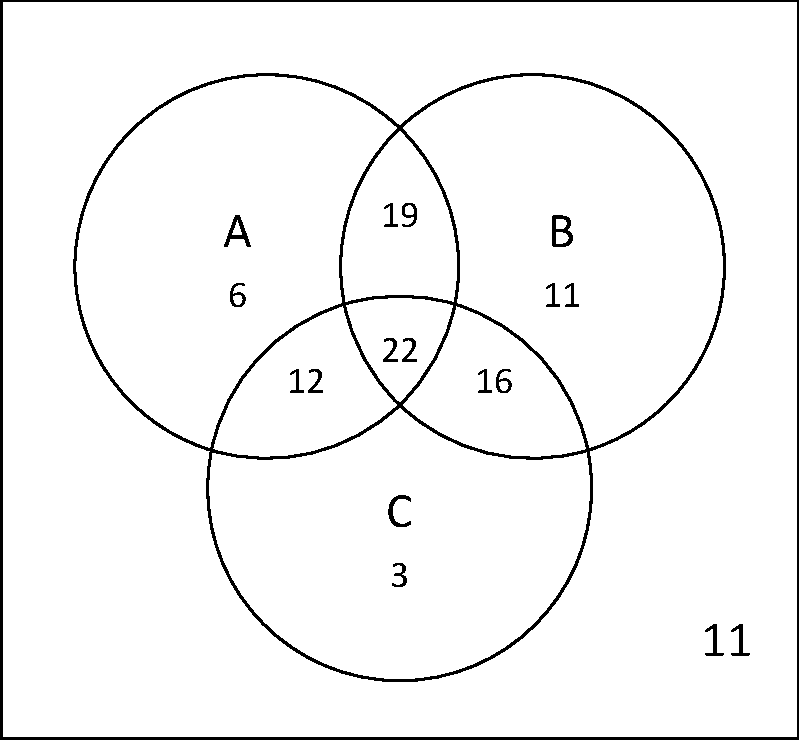
\includegraphics[scale=0.5]{./../img/venn_movies.pdf}
\end{figure}

\subsection{B) Hence find how many students watched}
\begin{quote}
\begin{enumerate}
\item Action and Calypso, but not Buzz
	\begin{itemize}
	\item 12
	\end{itemize}
\item Buzz only
	\begin{itemize}
	\item 11
	\end{itemize}
\item Only two of the three shows
	\begin{itemize}
	\item 47
	\end{itemize}
\item At least two of the shows
	\begin{itemize}
	\item 69
	\end{itemize}
\end{enumerate}
\end{quote}

\section{Question 3}

Suppose that $P$ is a set of people, and $M$ is a set of movies. Define the predicate $S(p, m)$ to mean ``person $p$ has seen movie $m$''. Consider the sentences below. For each sentence, the negation is also in the list. Match each sentence with its negation. Give your answer by listing the number of each sentence and its negation, for example ``4 and 10''.

\begin{enumerate}
\item There is at least one movie that some person has seen
	\begin{itemize}
	\item $\exists{m} \in{M}, \exists{p} \in{P}, S(p, m)$ % ∃m ∈ M, ∃p ∈ P, S(p, m)
	\end{itemize}
\item For each movie there is somebody who has not seen it
	\begin{itemize}
	\item $\forall{m} \in{M}, \exists{p} \in{P}, \sim{S}(p, m)$ % ∀m ∈ M, ∃p ∈ P, ~S(p, m)
	\end{itemize}
\item There is some movie that nobody has seen
	\begin{itemize}
	\item $\exists{m} \in{M}, \forall{p} \in{P}, \sim{S}(p, m)$ % ∃m ∈ M, ∀p ∈ P, ~S(p, m)
	\end{itemize}
\item There is at least one movie that everybody has seen
	\begin{itemize}
	\item $\exists{m} \in{M}, \forall{p} \in{P}, S(p, m)$ % ∃m ∈ M, ∀p ∈ P, S(p, m)
	\end{itemize}
\item For each movie there is somebody who has seen it
	\begin{itemize}
	\item $\forall{m} \in{M}, \exists{p} \in{P}, S(p, m)$ % ∀m ∈ M, ∃p ∈ P, S(p, m)
	\end{itemize}
\item There is some person who has not seen any of the movies
	\begin{itemize}
	\item $\exists{p} \in{P}, \forall{m} \in{M}, \sim{S}(p, m)$ % ∃p ∈ P, ∀m ∈ M, ~S(p, m)
	\end{itemize}
\item There is at least one movie that some person has not seen
	\begin{itemize}
	\item $\exists{m} \in{M}, \exists{p} \in{P}, \sim{S}(p, m)$ % ∃m ∈ M, ∃p ∈ P, ~S(p, m)
	\end{itemize}
\item Nobody has seen any of the movies
	\begin{itemize}
	\item $\forall{m} \in{M}, \forall{p} \in{P}, \sim{S}(p, m)$ % ∀m ∈ M, ∀p ∈ P, ~S(p, m)
	\end{itemize}
\item For each person there is some movie that they have not seen
	\begin{itemize}
	\item $\exists{p} \in{P}, \exists{m} \in{M}, \sim{S}(p, m)$ % ∃p ∈ P, ∃m ∈ M, ~S(p, m)
	\end{itemize}
\item Everybody has seen at least one movie
	\begin{itemize}
	\item $\forall{p} \in{P}, \exists{m} \in{M}, S(p, m)$ % ∀p ∈ P, ∃m ∈ M, S(p, m)
	\end{itemize}
\item There is some person who has seen all the movies
	\begin{itemize}
	\item $\exists{p} \in{P}, \forall{m} \in{M}, S(p, m)$ % ∃p ∈ P, ∀m ∈ M, S(p, m)
	\end{itemize}
\item Everybody has seen all of the movies
	\begin{itemize}
	\item $\forall{m} \in{M}, \forall{p} \in{P}, S(p, m)$ % ∀m ∈ M, ∀p ∈ P, S(p, m)
	\end{itemize}
\end{enumerate}

\subsection{Question 3 Answer}

\begin{enumerate}
\item 1 and 8
\item 2 and 4
\item 3 and 5
\item 6 and 10
\item 7 and 12
\item 9 and 11
\end{enumerate}

\section{Question 4}

\subsection{Introduction}

There is a simple way of representing sets using so-called \emph{bit strings}. A bit string is simply a string of 0's and 1's. Suppose that $U$ is the universal set. Then the rule for the bit string for a particular set $S$ is:
\\*
\\*
If the $k$th element of $U$ is in $S$, then the $k$th bit of the bit string is $1$. \\
If the $k$th element of $U$ is not in $S$, then the $k$th bit of the bit string is $0$.

\subsection{Example 1}
\begin{itemize}
\item Suppose the universal set is $U = \{1, 2, 3, 4, ..., 10\}$
\item Then set $A = \{1, 3, 5, 9\}$ is represented by the bit string $1010100010$
	\begin{itemize}
	\item The 1st element of $U$ appears in set $A$, so the 1st element of the bit string is $1$
	\item The 2nd element of $U$ does not appear in set $A$, so the 2nd element of the bit string is $0$
	\end{itemize}
\item The set $\{5, 6, 7\}$ is represented by bit string $0000111000$
\item Conversley, the bit string $0110010001$ represents the set $C = \{2, 3, 6, 10\}$
	\begin{itemize}		
	\item The 1st element of the bit string is $0$, so the 1st element of $U$ (which is $\{1\}$) is not in $C$
	\item The 2nd element of the bit string is $1$, so the 2nd element of $U$ (which is $\{2\}$) is in $C$
	\end{itemize}	
\item Similarly, the bit string $0000000110$ represents $\{8, 9\}$
\item And the bit string $0101010101$ represents $\{2, 4, 6, 8, 10\}$
\end{itemize}

\subsection{Example 2}

\begin{itemize}
\item The universal set is $U = \{4, 6, 9, 13, 18, 25\}$
\item Set $A = \{6, 13, 18\}$
\item Set $B = \{4, 13, 18, 25\}$
\end{itemize}
Suppose we want to find $A \cup B$, $A \cap B$ and $A'$. Using a table and performing the operations \textbf{bitwise}.

\begin{table}[h]
\centering
\caption{Question 4 Example 2 Truth Table}
\begin{tabular}{r|c|c|c|c|c|c}
$U$ & 4 & 6 & 9 & 13 & 18 & 25 \\
\hline
$A$ & 0 & 1 & 0 & 1 & 1 & 0 \\
\hline
$B$ & 1 & 0 & 0 & 1 & 1 & 1 \\
\hline
$A \cup B$ & 1 & 1 & 0 & 1 & 1 & 1 \\
\hline
$A \cap B$ & 0 & 0 & 0 & 1 & 1 & 0 \\
\hline
$A'$ & 1 & 0 & 1 & 0 & 0 & 1 \\
\hline
\end{tabular}
\end{table}
From the table we get:
\begin{itemize}
\item $A \cup B$ bit string is $110111$
	\begin{itemize}
	\item $A \cup B = \{4, 6, 13, 18, 25\}$
	\end{itemize}
\item $A \cap B$ bit string is $000110$
	\begin{itemize}
	\item $A \cap B = \{13, 18\}$
	\end{itemize}
\item $A'$ bit string is $101001$
	\begin{itemize}
	\item $A' = \{4, 9, 25\}$
	\end{itemize}
\end{itemize}

\subsection{Task}
\begin{gather*}
U = \{Argentina, Australia, Belgium, Brazil, Cameroon, Chile, Cuba, Denmark, Egypt, 
\\Ethiopia, Fiji, France, Germany, Ghana, Greece, Haiti\}
\end{gather*}

\begin{enumerate}
\item Find the bit string that represents the set $L = \{Brazil, Fiji, Ghana, Greece\}$
	\begin{itemize}
	\item Bit string $L$ = 0001 0000 0010 0110
	\end{itemize}
\item Find the set $M$ represented by bit string 0000 0110 1001 0001
	\begin{itemize}
	\item $M = \{Chile, Cuba, Egypt, France, Haiti\}$
	\end{itemize}
\item Let $P$, $Q$, $R$ and $S$ be sets represented by the following bit strings respectively (see Table 7)
	\begin{itemize}
	\item Find the bit string that represent the set $T = (P \cap Q') \cup (R' \cap S)$
		\begin{itemize}
		\item Bit string $T$ = 1000 0010 1010 0100
		\end{itemize}
	\end{itemize}
\item List the countries in the set $T$
	\begin{itemize}
	\item T = $\{Argentina, Cuba, Egypt, Fiji, Ghana\}$
	\end{itemize}
\end{enumerate}

\newpage
\begin{landscape}
\thispagestyle{fancylscape}
\begin{table}[h]
\centering
\caption{Question 4 Task Truth Table}
\begin{tabular}{r|c|c|c|c|c|c|c|c|c|c|c|c|c|c|c|c}
$U$ & Ar & Au & Be & Br & Ca & Ch & Cu & De & Eg & Et & Fi & Fr & Ge & Gh & Gr & Ha \\
\hline
$L$ & 0 & 0 & 0 & 1 & 0 & 0 & 0 & 0 & 0 & 0 & 1 & 0 & 0 & 1 & 1 & 0 \\
\hline
$M$ & 0 & 0 & 0 & 0 & 0 & 1 & 1 & 0 & 1 & 0 & 0 & 1 & 0 & 0 & 0 & 1 \\
\hline
$P$ & 1 & 1 & 0 & 1 & 0 & 1 & 0 & 0 & 1 & 0 & 1 & 0 & 1 & 1 & 1 & 0 \\
\hline
$Q$ & 0 & 1 & 1 & 1 & 1 & 1 & 0 & 0 & 0 & 1 & 0 & 0 & 1 & 0 & 1 & 1 \\
\hline
$R$ & 0 & 1 & 0 & 1 & 1 & 1 & 0 & 1 & 1 & 0 & 0 & 1 & 1 & 0 & 0 & 1 \\
\hline
$S$ & 1 & 1 & 0 & 1 & 0 & 0 & 1 & 1 & 0 & 1 & 1 & 0 & 1 & 0 & 0 & 1 \\
\hline
$Q'$ & 1 & 0 & 0 & 0 & 0 & 0 & 1 & 1 & 1 & 0 & 1 & 1 & 0 & 1 & 0 & 0 \\
\hline
$P \cap Q'$ & 1 & 0 & 0 & 0 & 0 & 0 & 0 & 0 & 1 & 0 & 1 & 0 & 0 & 1 & 0 & 0 \\
\hline
$R'$ & 1 & 0 & 1 & 0 & 0 & 0 & 1 & 0 & 0 & 1 & 1 & 0 & 0 & 1 & 1 & 0 \\
\hline
$R' \cap S$ & 1 & 0 & 0 & 0 & 0 & 0 & 1 & 0 & 0 & 1 & 1 & 0 & 0 & 0 & 0 & 0 \\
\hline
$T$ & 1 & 0 & 0 & 0 & 0 & 0 & 1 & 0 & 1 & 0 & 1 & 0 & 0 & 1 & 0 & 0 \\
\end{tabular}
\end{table}
\end{landscape}

\newpage
\section{Question 5}
In lecture notes there is an application of Karnaugh maps to a 7-segment display that is used in some calculators and similar digital devices. The display is sometimes \emph{extended} to include \emph{all} hexadecimal digits. A typical extended display is:

\begin{figure}[h]
\centering
\caption{7-Segment Characters}
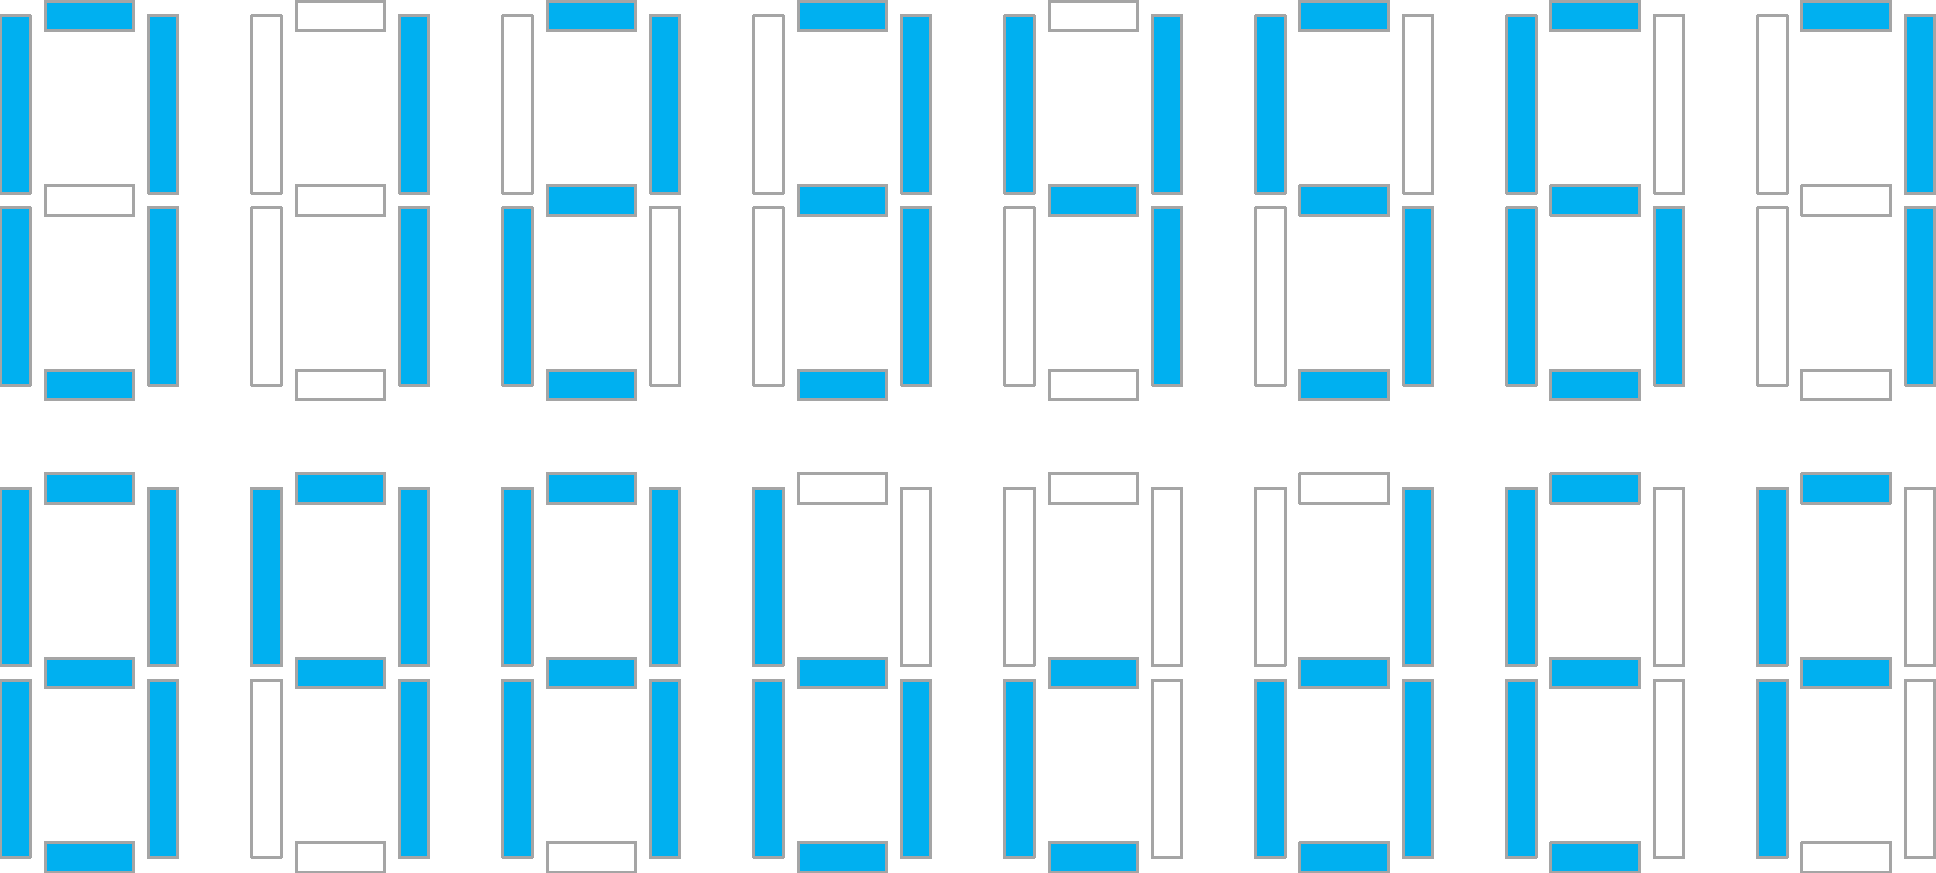
\includegraphics[scale=0.5]{./../img/7-seg-chars.pdf}
\end{figure}
Notice the display for the hexidecimal digits for 10 through 15. Some are shown as upper case and some lower case: A, b, c, d, E, F. As in the lecture notes we label each of the seven segments as shown:

\begin{figure}[h]
\centering
\caption{7-Segment Segments}
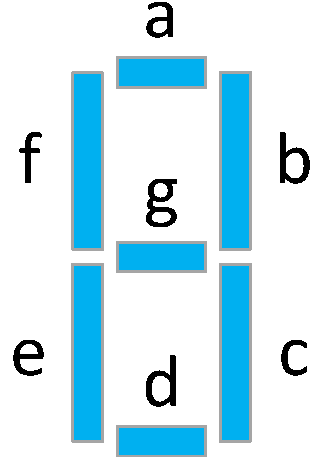
\includegraphics[scale=0.5]{./../img/7-seg-segments.pdf}
\end{figure}
When any of the keys, 0, 1, 2, 3, 4, 5, 6, 7, 8, 9, A, B, C, D, E, F is pressed, a 4-bit binary signal $wxyz$ is generated, as shown in Table 8.
\\
\\
For each of the seven segments, there is a corresponding Boolean function and a circuit that has output 0 or 1 as the various keys are pressed. Denote these functions by $a(w,x,y,z)$, $a(w,x,y,z)$, ..., $g(w,x,y,z)$.

\newpage
\subsection{Task}
Your task concerns the two segments $d$ and $g$, and is as follows. For \textbf{each} of the two functions $d(w,x,y,z)$ and $g(w,x,y,z)$:

\subsubsection{Construct a truth table for functions $d(w,x,y,z)$ and $g(w,x,y,z)$}

\begin{table}[h]
\centering
\caption{Question 5 Task Truth Table}
\begin{tabular}{c|c|c|c|c|c|c|c|c|c|c|c}
Key & w & x & y & z & a & b & c & d & e & f & g \\
\hline
0 & 0 & 0 & 0 & 0 & 1 & 1 & 1 & 1 & 1 & 1 & 0 \\
\hline
1 & 0 & 0 & 0 & 1 & 0 & 1 & 1 & 0 & 0 & 0 & 0 \\
\hline
2 & 0 & 0 & 1 & 0 & 1 & 1 & 0 & 1 & 1 & 0 & 1 \\
\hline
3 & 0 & 0 & 1 & 1 & 1 & 1 & 1 & 1 & 0 & 0 & 1 \\
\hline
4 & 0 & 1 & 0 & 0 & 0 & 1 & 1 & 0 & 0 & 1 & 1 \\
\hline
5 & 0 & 1 & 0 & 1 & 1 & 0 & 1 & 1 & 0 & 1 & 1 \\
\hline
6 & 0 & 1 & 1 & 0 & 1 & 0 & 1 & 1 & 1 & 1 & 1 \\
\hline
7 & 0 & 1 & 1 & 1 & 1 & 1 & 1 & 0 & 0 & 0 & 0 \\
\hline
8 & 1 & 0 & 0 & 0 & 1 & 1 & 1 & 1 & 1 & 1 & 1 \\
\hline
9 & 1 & 0 & 0 & 1 & 1 & 1 & 1 & 0 & 0 & 1 & 1 \\
\hline
A & 1 & 0 & 1 & 0 & 1 & 1 & 1 & 0 & 1 & 1 & 1 \\
\hline
B & 1 & 0 & 1 & 1 & 0 & 0 & 1 & 1 & 1 & 1 & 1 \\
\hline
C & 1 & 1 & 0 & 0 & 0 & 0 & 0 & 1 & 1 & 0 & 1 \\
\hline
D & 1 & 1 & 0 & 1 & 0 & 1 & 1 & 1 & 1 & 0 & 1 \\
\hline
E & 1 & 1 & 1 & 0 & 1 & 0 & 0 & 1 & 1 & 1 & 1 \\
\hline
F & 1 & 1 & 1 & 1 & 1 & 0 & 0 & 0 & 1 & 1 & 1 \\
\end{tabular}
\end{table}

\newpage
\subsubsection{Construct the corresponding Karnaugh map}
Use the \emph{simple} labelling on the Karnaugh maps and show your groups clearly.

\begin{figure}[h]
\centering
\caption{$d(w,x,y,z)$ Karnaugh map}
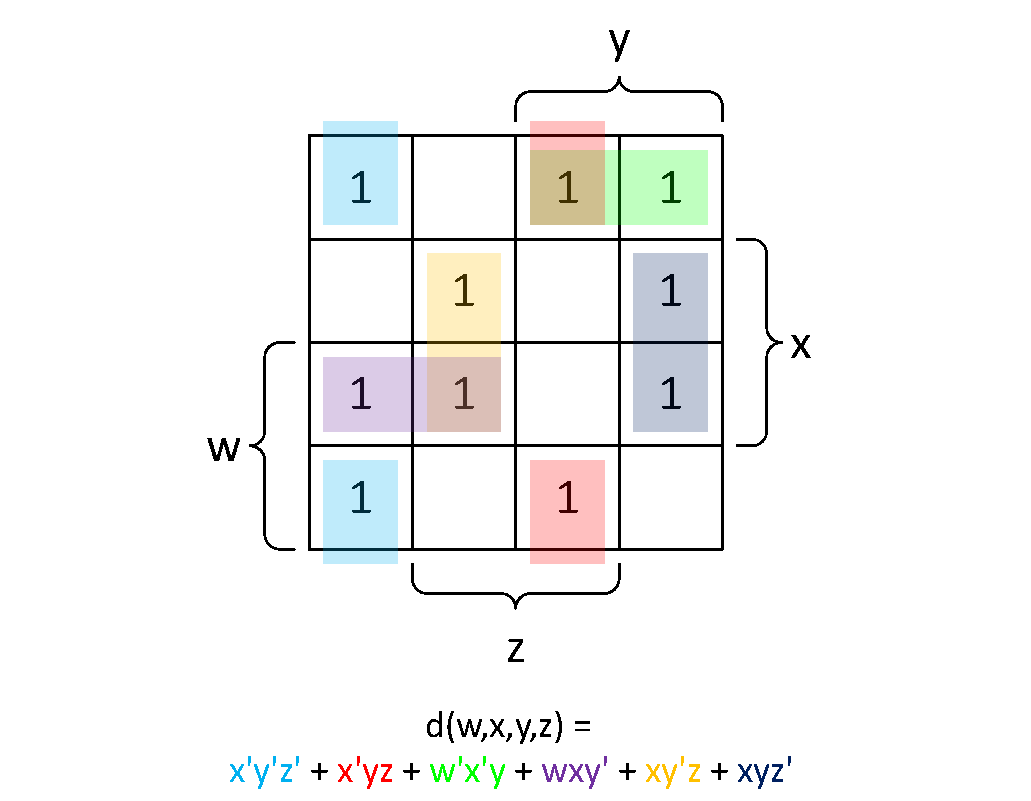
\includegraphics[scale=0.56]{./../img/q5-2_d.pdf}
\end{figure}

\begin{figure}[h]
\centering
\caption{$g(w,x,y,z)$ Karnaugh map}
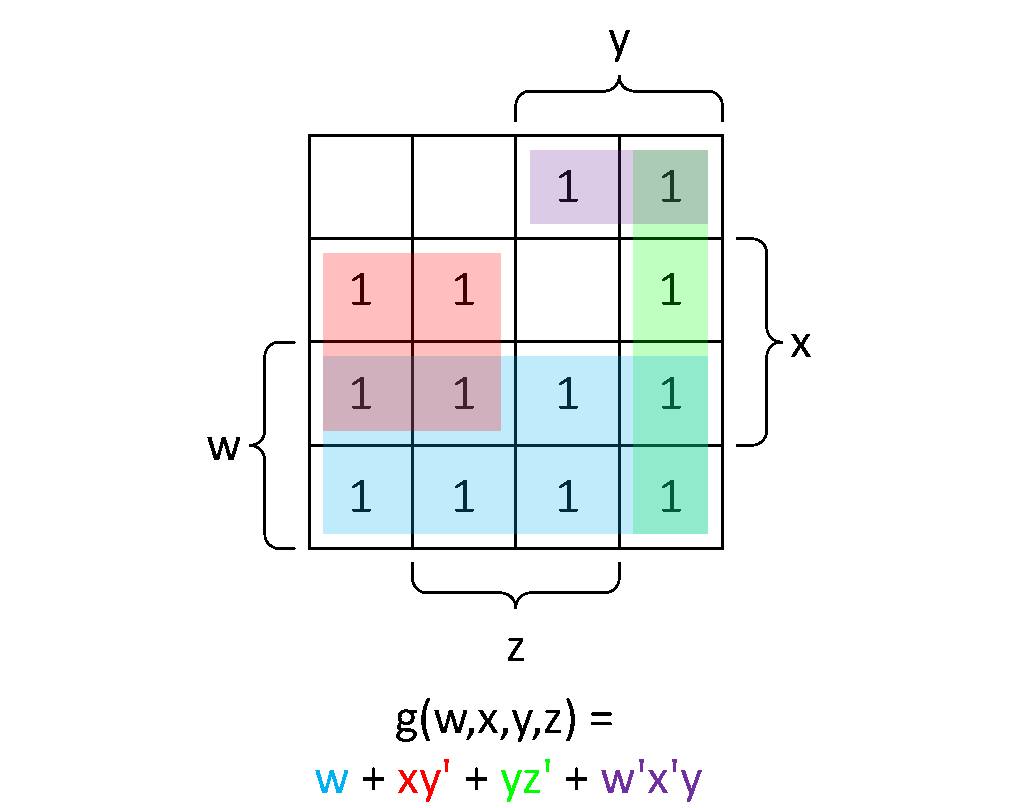
\includegraphics[scale=0.56]{./../img/q5-2_g.pdf}
\end{figure}

\subsubsection{Find the minimal sum of products for the functions}
\begin{align*}
d(w,x,y,z) &= x'y'z' + x'yz + w'x'y + wxy' + xy'z + xyz' \\
g(w,x,y,z) &= w + xy' + yz' + w'x'y
\end{align*}

\end{document}